% Solution: Tadelis (2013) Exercise 6.5 "Cops and Robbers". Input by \solitem.
% New in the Lecture 3 practice list. Check: check_L03.py.
\begin{exsol}{Tadelis Exercise 6.5}{124}{Foundations}{2}
\asked A police officer (player~1) chooses between patrolling the streets and the coffee shop; a
robber (player~2) chooses between staying hidden and prowling. (a) Write the matrix; (b) draw each
player's best-response function; (c) find the Nash equilibrium and say which game it recalls.

\method Build the matrix from the story, mark best replies, and, because every cell is a best reply of
at most one player, look for an equilibrium in mixed strategies with the principle of indifference
(Lecture~3, slides~21--26 and the battle of the sexes on slides~27--34; Tadelis \S6.2, pp.~108--114).

\solution
\textbf{(a) Matrix.} Let $P$ = patrol, $C$ = coffee shop for player~1 and $H$ = hidden, $S$ = prowl
the streets for player~2. Coffee shop pays the officer 10 whatever the robber does; patrolling pays
20 if the robber prowls and 0 if he hides. The robber gets 0 hidden; if he prowls he gets $-10$ against
a patrol and 10 against the coffee shop.
\begin{center}
\begin{tabular}{r|c|c|}
\multicolumn{1}{r}{} & \multicolumn{1}{c}{$H$} & \multicolumn{1}{c}{$S$}\\ \cline{2-3}
$P$ & $0,\ \br{0}$ & $\br{20},\ -10$ \\ \cline{2-3}
$C$ & $\br{10},\ 0$ & $10,\ \br{10}$ \\ \cline{2-3}
\end{tabular}
\end{center}
Underlined payoffs are best replies. No cell has both payoffs underlined, so there is no pure Nash
equilibrium: the replies chase each other around the matrix. Against
$H$ the officer prefers $C$, against $C$ the robber prefers $S$, against $S$ the officer prefers $P$,
against $P$ the robber prefers $H$.

\textbf{(b) Best-response functions.} Let $p = \Pr(P)$ and $q = \Pr(S)$. Expected payoffs:
\begin{align*}
  u_1(P, q) &= 20q, & u_1(C, q) &= 10, \\
  u_2(H, p) &= 0, & u_2(S, p) &= -10p + 10(1-p) = 10 - 20p.
\end{align*}
The officer prefers $P$ iff $20q > 10$, i.e.\ $q > \frac12$; the robber prefers $S$ iff $10 - 20p > 0$,
i.e.\ $p < \frac12$. Hence
\[
  BR_1(q) = \begin{cases} p = 0 & q < \frac12\\ p \in [0,1] & q = \frac12\\ p = 1 & q > \frac12\end{cases},
  \qquad
  BR_2(p) = \begin{cases} q = 1 & p < \frac12\\ q \in [0,1] & p = \frac12\\ q = 0 & p > \frac12\end{cases}.
\]
\begin{center}
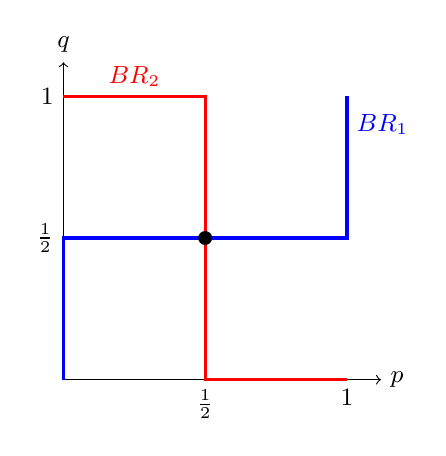
\begin{tikzpicture}[scale=3.6,font=\small]
  \draw[->] (0,0) -- (1.12,0) node[right] {$p$};
  \draw[->] (0,0) -- (0,1.12) node[above] {$q$};
  \node[below] at (1,0) {1}; \node[left] at (0,1) {1};
  \node[below] at (0.5,0) {$\frac12$}; \node[left] at (0,0.5) {$\frac12$};
  \draw[very thick,blue] (0,0) -- (0,0.5) -- (1,0.5) -- (1,1);
  \draw[very thick,red] (0,1) -- (0.5,1) -- (0.5,0) -- (1,0);
  \fill (0.5,0.5) circle (0.7pt);
  \node[blue,right] at (1,0.9) {$BR_1$};
  \node[red,above] at (0.25,1) {$BR_2$};
\end{tikzpicture}
\end{center}
The two graphs cross once, at $(p,q) = (\frac12,\frac12)$.

\textbf{(c) Nash equilibrium.} Indifference of the robber: $0 = 10 - 20p$ gives $p = \frac12$;
indifference of the officer: $20q = 10$ gives $q = \frac12$. The unique Nash equilibrium is
\[
  \sigma^* = \bigl(\tfrac12 P + \tfrac12 C,\ \ \tfrac12 H + \tfrac12 S\bigr),
\]
with expected payoffs $u_1 = 10$ and $u_2 = 0$. It is unique because no pure strategy of either player
is a best reply to a pure strategy of the other, and a mixed equilibrium with one player pure is
ruled out by the best-reply functions above (a pure $p$ makes the robber strictly prefer one pure
action, which makes the officer strictly prefer one pure action, which breaks the first).

The game recalls \emph{matching pennies} (and the penalty kick of slide~3): one player wants to
match the other's action, the other wants to mismatch, so each must be unpredictable. It is an
inspection game rather than a zero-sum game (payoffs do not sum to a constant), but the logic is the same.

\interp The equilibrium probabilities are set by the \emph{other} player's payoffs: the officer
patrols half the time because that is what makes the robber indifferent, not because patrolling is
attractive in itself. If the robber's fine for being caught grew from $10$ to $20$ (payoff $-20$ against a
patrol), $u_2(S,p) = 10 - 30p$ and the officer would patrol only a third of the time; the officer
itself is unaffected in equilibrium (still 10).

\verify \texttt{check\_L03.py} finds no pure equilibrium, solves both indifference equations
exactly, checks that $(\frac12,\frac12)$ is a Nash equilibrium against all pure deviations, finds it is
the only mixed equilibrium by support enumeration, and recomputes the patrol probability
$\frac13$ in the larger-fine variant. Output line: \texttt{tadelis-6-5: no pure NE; mixed NE
(1/2,1/2), payoffs (10, 0)}. Tadelis prints no answer.

\mistakes
\begin{itemize}
  \item Computing the officer's mix from the \emph{officer's} indifference: it makes the officer
  indifferent, not the robber, and gives $q$, the robber's probability.
  \item Reporting the equilibrium payoff of the officer as $20 \cdot \frac12 = 10$ from patrolling only,
  or forgetting that the robber's expected payoff is exactly $0$ (his payoff from hiding).
  \item Stopping at ``no equilibrium'': there is no equilibrium \emph{in pure strategies}; Nash's theorem
  gives one in mixed strategies.
\end{itemize}

\answer{(a) The matrix above ($P,H$: $(0,0)$; $P,S$: $(20,-10)$; $C,H$: $(10,0)$; $C,S$: $(10,10)$).
(b) $BR_1$ switches at $q = \frac12$, $BR_2$ at $p = \frac12$. (c) No pure equilibrium; the unique
Nash equilibrium is mixed, $p = \Pr(\text{patrol}) = \frac12$, $q = \Pr(\text{prowl}) = \frac12$,
with payoffs $(10, 0)$; the game resembles matching pennies.}
\end{exsol}
